\documentclass[sigplan,screen,review,anonymous,nonacm]{acmart}

\setcopyright{none}
\settopmatter{printacmref=false, printccs=false, printfolios=true}
\renewcommand\footnotetextcopyrightpermission[1]{}
\pagestyle{plain}

\usepackage{booktabs}
\graphicspath{{figures/}}

\title{Graduated Action Routing for ReAct Agents:\\
Measuring 8B Usage--Accuracy Tradeoffs Across an SLM--LLM Cascade}

\author{Anonymous Author(s)}
\affiliation{
  \institution{Anonymous Institution}
  \country{Anonymous}
}

\begin{abstract}
Agentic engineering needs runtime controls that make agent behavior reliable
without routing every action through the largest available model.
Language-model cascades are one candidate control: they aim to reduce inference cost by
routing requests between small and large models. For agents, however, the
natural routing unit is not only the request. A ReAct trajectory is a sequence
of action decisions, and a weak model may be adequate for some steps but not
others. We study per-action routing in ReAct-style multi-hop question-answering
agents using open-weight 1.5B/3B/8B model tiers. Across 20,500 episodes on
HotpotQA and MuSiQue, we compare 41 routing policies spanning confidence
gates, entropy gates, step gates, three-level cascades, and a learned
logit-feature router. The results are cautionary. First-token entropy is the
strongest of the tested uncertainty gates on the usage--accuracy frontier:
no tested policy reaches 90\% of the always-8B baseline below 60\%
8B-call ratio. The tested confidence gate is not competitive. A learned router reaches in-sample AUC 0.71 on logged
steps but is Pareto-dominated when deployed online. In contrast, simple
structural policies are strong: keeping the 1.5B model for the first action
and escalating later obtains similar observed accuracy to always-8B at a
mean per-episode 8B-step fraction of about 76--79\%. A 1.5B--3B--8B cascade
improves observed accuracy over always-3B with very little 8B usage.
These fractions do not measure total inference cost or relative call counts.
These results support a measurement-first approach to cost-aware reliability
controls for language-agent runtimes.
\end{abstract}

\keywords{agentic engineering, LLM agents, model routing, cascades, ReAct, uncertainty, efficient inference}

\begin{document}
\maketitle

\section{Introduction}

Large language model (LLM) agents can operate as multi-step
systems: they plan, call tools, observe results, and decide whether to stop or
continue \cite{react,redact,evoroute}. From an agentic-engineering perspective, this raises a runtime
control question: how should an agent spend stronger model calls only where
they improve reliability? A single difficult question may contain easy and hard
action decisions, and routing the whole query to one model can either
overspend on routine steps or underspend on steps where an early error derails
the rest of the episode.

Prior work studies request-level model selection and cascades
\cite{frugalgpt,routellm,hybridllm}. More recent work studies step-level
routing for mathematical reasoning or agentic environments
\cite{trim,redact,evoroute,tacitswitch}. Our goal is complementary: we
perform a controlled empirical audit of action-level routing inside a
ReAct-style question-answering agent, using small open-weight model tiers and
end-to-end task success rather than offline routing metrics alone.

The study asks a practical question for trustworthy and cost-aware agent
runtimes: \emph{when does it actually pay to escalate a ReAct action from a
small language model (SLM) to a larger model?}
We evaluate six policy families over HotpotQA and MuSiQue: always-small and
always-large baselines, verbalized-confidence gates, first-token entropy
gates, step-index gates, a three-level 1.5B--3B--8B cascade, and a logistic
learned router trained on logit features. Each policy is evaluated online in
the agent loop, so routing decisions affect later observations and future
steps.

Our findings are intentionally not a simple ``routing works'' story:

\begin{itemize}
  \item We confirm substantial headroom between a 1.5B ReAct agent and an 8B
  baseline: 0.053 vs. 0.273 exact match on HotpotQA and 0.005 vs. 0.195 on
  MuSiQue.
  \item Among cheap uncertainty signals, first-token entropy is useful and
  the tested confidence gate is not competitive. Entropy routing does not meet a
  target of 90\% always-8B success below a 60\% mean 8B-step fraction.
  \item Structural routing is unexpectedly strong. The first ReAct action is
  low-entropy for the SLM, while later actions are high-entropy; keeping the
  SLM for step 0 and escalating afterward obtains similar observed accuracy
  to always-8B. This does not establish statistical equivalence.
  \item A learned router can look promising offline yet fail online: the
  deployed logit-feature router has training-set AUC 0.71 on logged steps but is
  Pareto-dominated across thresholds.
  \item A mid-tier cascade changes the low-8B-usage regime, producing
  higher observed accuracy than always-3B with near-zero 8B usage in its
  best settings. The episode logs do not separately count executed 3B steps.
\end{itemize}

Together, these results argue that action routing for agents should be judged
by online task-level frontiers, not only by uncertainty AUC or isolated step
classifiers.

\section{Related Work}

\paragraph{Query-level model routing.}
LLM cascades route requests to cheaper or stronger models to trade quality for
cost. FrugalGPT uses cascades to reduce API cost while preserving response
quality \cite{frugalgpt}; RouteLLM learns routers from preference data
\cite{routellm}; Hybrid LLM studies quality-aware query routing
\cite{hybridllm}. These systems operate at request granularity; a cascade may invoke
several models for one request. That is a
natural abstraction for single-turn tasks, but agents expose a finer decision
surface: each trajectory contains multiple action choices whose difficulty may
vary.

\paragraph{Agentic and step-level routing.}
Recent work has begun to route within trajectories. TRIM routes critical
reasoning steps in multi-step math tasks using process-reward information and
budget-aware policies \cite{trim}. ReDAct studies uncertainty-aware deferral
for LLM agents in sequential environments, where a small model defers action
decisions to a larger model under high uncertainty \cite{redact}. EvoRoute
selects LLM backbones at steps in complex agent systems using accumulated
experience \cite{evoroute}. TACIT-Switch learns cost-aware handoff policies
from censored supervision and compares task-level, prefix, and local switching
\cite{tacitswitch}. Our study differs in its setting and emphasis: we focus on
ReAct-style multi-hop QA with open-weight 1.5B/3B/8B tiers, compare simple
signals and structural policies under the same environment, and foreground
negative online results for confidence and learned routing.

\paragraph{Uncertainty and confidence signals.}
Lin et al.\ study learned verbalized uncertainty and compare it with
logit-derived uncertainty \cite{verbalized}. Our confidence gate instead
prompts an instruction-tuned model without additional calibration training. For action routing, the important distinction is not only
whether a signal predicts failure offline, but whether thresholding that signal
improves the online cost--quality frontier. Our results support this
distinction: first-token entropy has modest offline discrimination and useful
online behavior; the tested confidence gate is weak; and a learned logit router
with training-set AUC above 0.70 still fails to produce a competitive routing policy.

\paragraph{ReAct and multi-hop QA.}
ReAct agents interleave reasoning traces and tool actions
\cite{react}. HotpotQA and MuSiQue provide multi-hop QA benchmarks with
supporting passages and distractors \cite{hotpotqa,musique}. We use these
benchmarks not to claim state-of-the-art QA performance, but to study routing
behavior in a controlled tool-using setting where step-level choices affect
retrieval observations and downstream termination.

\section{Experimental Setup}
\label{sec:setup}

\subsection{Agent Environment}

We evaluate ReAct-style agents \cite{react} for multi-hop question answering. At each step,
the agent receives the question and a scratchpad of prior
Thought--Action--Observation triples, then emits a Thought and either a
\texttt{Search[query]} action or a \texttt{Finish[answer]} action. Search uses
BM25 \cite{bm25} over the current question's candidate passages. The top two
passages are concatenated and truncated to 500 characters for the observation. Episodes are capped at eight steps and are
scored by exact match after lowercasing, article removal, punctuation removal,
and whitespace normalization.

All decoding is greedy, with at most 256 new tokens per action and input
truncation at 2,048 tokens. On routed policies, the 1.5B model always generates
the candidate step first so that logits and text are available to the router.
If the router escalates, the selected larger model regenerates the same step.
For episode $i$, let $L_i$ count executed 8B steps and $S_i$ all executed
steps. We report $N^{-1}\sum_{i=1}^{N} L_i/S_i$, the mean per-episode
8B-step fraction (\texttt{llm\_call\_ratio}). This is neither the pooled
fraction of steps nor the call count relative to always-8B. It excludes
candidate generations, confidence elicitation, and intermediate 3B calls.
The always-8B runner also generates twice with the same 8B model per step
but records one executed step. We measure tier usage, not actual compute
savings, latency, or monetary cost.

\subsection{Models}

Table~\ref{tab:models} lists the model tiers. The 1.5B model is the default
actor. The 3B model is used as a standalone baseline and in the cascade.
The Qwen tiers use Qwen2.5-Instruct \cite{qwen25}; the 8B tier uses
Llama-3.1-Instruct \cite{llama3}. Always-8B is a reference, not an oracle
or upper bound: mixed policies can exceed its observed accuracy.
The experiment scripts load models in FP16.

\begin{table}[t]
\caption{Model tiers used in the routing cascade.}
\label{tab:models}
\centering
\begin{tabular}{llll}
\toprule
Tier & Checkpoint & Params & Role \\
\midrule
SLM & Qwen2.5-Instruct & 1.5B & Default actor \\
Mid & Qwen2.5-Instruct & 3B & Cascade tier \\
LLM & Llama-3.1-Instruct & 8B & Escalation \\
\bottomrule
\end{tabular}
\end{table}

\subsection{Datasets}

We use the first 300 HotpotQA distractor validation questions \cite{hotpotqa}
and first 200 MuSiQue validation questions \cite{musique}, in loader order. HotpotQA examples contain roughly ten candidate passages per
question; MuSiQue examples contain roughly twenty. Retrieval is deliberately
per-question: each example builds a BM25 index over its own candidate passage
set, so retrieval difficulty is tied to the example rather than to open-corpus
search.

\subsection{Routing Policies}

Table~\ref{tab:policies} summarizes the 41 policies evaluated on both
datasets. The confidence gate asks the SLM for a verbalized confidence score
and escalates when the score is below a threshold. The entropy gate escalates
when the first generated token's entropy exceeds a threshold. The step gate
escalates all steps with index at least $k$. The three-level cascade first
routes from 1.5B to 3B using entropy, then from 3B to 8B using the 3B model's
own entropy. The learned router is logistic regression over five logit
features: first-token entropy, mean entropy, top-1 probability, top-1--top-2
margin, and mean top-5 probability. It is trained on 1,859 1.5B baseline
steps using the episode-level label ``this step belongs to a failed episode''
as a proxy for needing escalation. Features are standardized, with
class-balanced logistic regression ($C=1$, 500 maximum iterations).
Training pools both datasets; AUC is computed on the training steps, and
online evaluation reuses the same questions. There is no held-out split.

Confidence thresholds are $0.1,0.2,\ldots,0.9$; entropy thresholds are
$0.5,1.0,\ldots,4.0$ nats; step gates use $k=1,\ldots,6$ with zero-based
step indices; and learned-router thresholds are $0.2,0.3,\ldots,0.8$.
The cascade tests $(t_1,t_2)$ pairs $(0.5,1.5)$, $(0.5,2.0)$,
$(0.5,2.5)$, $(1.0,2.0)$, $(1.0,2.5)$, $(1.0,3.0)$,
$(1.5,2.5)$, and $(1.5,3.0)$, with both entropies measured in nats.
Unparseable confidence responses trigger escalation. These settings define
the scope of the sweep; no claim covers untested thresholds or policies.

\begin{table}[t]
\caption{Routing policy families.}
\label{tab:policies}
\centering
\begin{tabular}{lll}
\toprule
Family & Signal & Configs \\
\midrule
Always SLM/LLM & none & 3 \\
Confidence gate & verbalized confidence & 9 \\
Entropy gate & first-token entropy & 8 \\
Step gate & step index & 6 \\
Three-level cascade & two-stage entropy & 8 \\
Learned router & logit features & 7 \\
\bottomrule
\end{tabular}
\end{table}

\subsection{Hypotheses}

We assess three experimental criteria, labelled H0--H2 in the project notes. H0: a capability gap exists, i.e.,
the always-8B baseline outperforms the 1.5B baseline on both datasets. H1: some routing
policy reaches at least 90\% of always-8B success at below 60\% 8B-call ratio.
H2: at least one uncertainty-based policy lies on the usage--accuracy Pareto frontier. The
experiments cover 82 dataset-policy configurations and 20,500 total episodes.

\section{Results}
\label{sec:results}

\subsection{Baseline Capability Gap}

Table~\ref{tab:baselines} shows the baseline success rates. H0 passes: the 8B
baseline has higher observed accuracy than the 1.5B baseline on both datasets. The 3B model also
improves over 1.5B, showing that a middle tier has real value before invoking
the 8B model.

\begin{table}[t]
\caption{Baseline exact-match success rates.}
\label{tab:baselines}
\centering
\begin{tabular}{lcc}
\toprule
Policy & HotpotQA & MuSiQue \\
\midrule
Always 1.5B & 0.053 & 0.005 \\
Always 3B & 0.143 & 0.045 \\
Always 8B & 0.273 & 0.195 \\
\bottomrule
\end{tabular}
\end{table}

\subsection{Entropy Gating Improves Accuracy with Higher 8B Usage}

Figure~\ref{fig:pareto} shows the HotpotQA policy sweep. Entropy gating
contributes non-dominated points on each dataset's usage--accuracy frontier,
satisfying H2 among the evaluated configurations. The best policy below
60\% 8B-call ratio is
entropy threshold 2.0, which reaches 0.210 success on HotpotQA and 0.145 on
MuSiQue. These are 77\% and 74\% of the respective always-8B rates, below the
90\% target. H1 therefore fails on both datasets.

\begin{figure}[t]
  \centering
  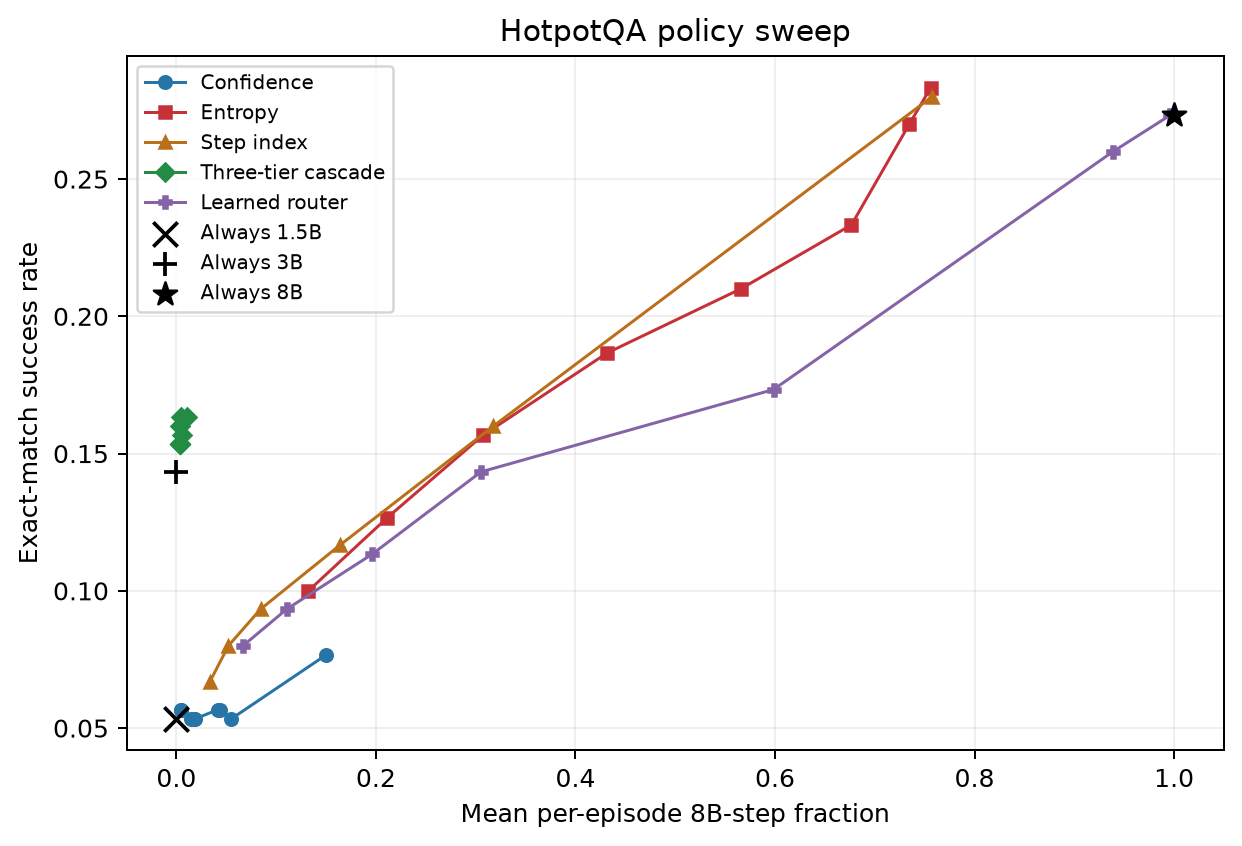
\includegraphics[width=\linewidth]{fig1_pareto_frontier.png}
  \caption{Usage--accuracy sweep on HotpotQA. Lines connect evaluated settings
  for visual guidance, not measured intermediate policies. Entropy gating is the strongest
  uncertainty family, but no uncertainty policy reaches 90\% of always-8B success
  below 60\% 8B-call ratio.}
  \label{fig:pareto}
\end{figure}

The confidence gate is not competitive. Its best HotpotQA point is 0.077
success at 0.150 8B-call ratio, and its best MuSiQue point is 0.030 at 0.247.
This prompted confidence gate is weak on these questions; we do not infer
that calibrated or differently elicited confidence is generally ineffective.

\subsection{A Simple Step Gate Is Competitive}

The step gate reveals a simple structure in the trajectories. Escalating from
step 1 onward, while keeping the SLM for the first step, obtains 0.280 on
HotpotQA and 0.220 on MuSiQue at about 0.76--0.79 8B-call ratio. The corresponding always-8B rates are 0.273 and 0.195. These are descriptive
comparisons on the same questions, not evidence of equivalence or a
statistically established improvement. Confirmatory comparisons should use
paired question-level tests and confidence intervals.

Figure~\ref{fig:steps} shows an associated signal pattern. Mean first-token
entropy is 0.190 on HotpotQA and 0.197 on MuSiQue at step 0, rising to
approximately 2.94--3.41 at later steps. Fewer than half of baseline episodes
remain active at step index 3. Low entropy does not establish correctness:
the first generated token can reflect the required response format rather
than semantic certainty. These logs do not establish why the step gate works.

\begin{figure*}[t]
  \centering
  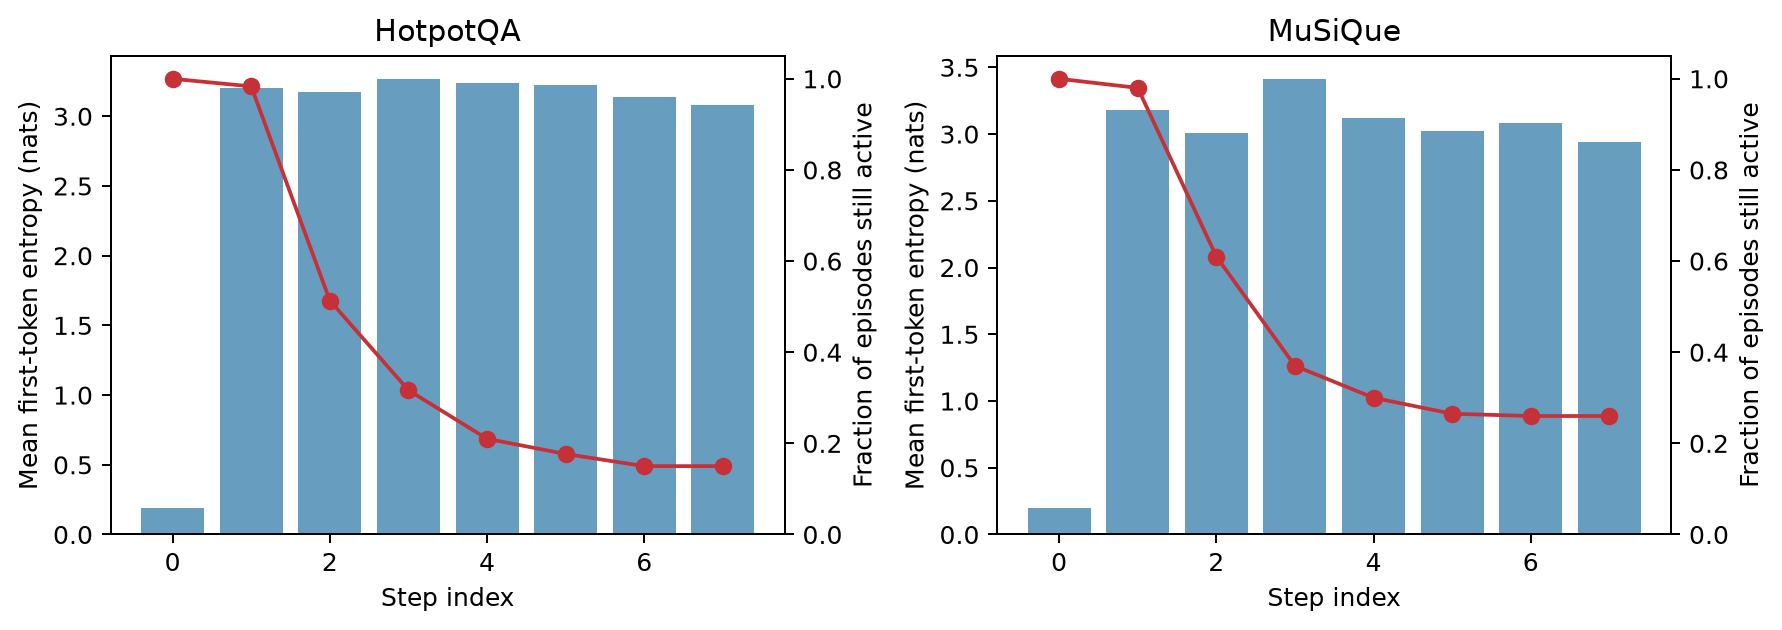
\includegraphics[width=0.85\textwidth]{fig3_step_escalation.png}
  \caption{Step-level signals for the 1.5B baseline. Bars show mean
  first-token entropy by step; the red curve shows the fraction of episodes
  still active. Later steps have higher first-token entropy; this is not a
  direct measure of action correctness.}
  \label{fig:steps}
\end{figure*}

\subsection{A Mid-Tier Cascade Reduces 8B Usage}

Figure~\ref{fig:cascade} shows that the three-level cascade occupies a region that two-level entropy gating does
not: it improves over the 3B baseline while using almost no 8B calls. On
HotpotQA, the best cascade reaches 0.163 success at 0.004 8B-call ratio,
compared with 0.143 for always-3B. On MuSiQue, it reaches 0.080 at essentially
zero 8B usage, compared with 0.045 for always-3B. These gains should be read
as promising but sample-limited. These points establish low 8B usage,
not low total cost; a larger confirmatory run should test the effect size.

\begin{figure}[t]
  \centering
  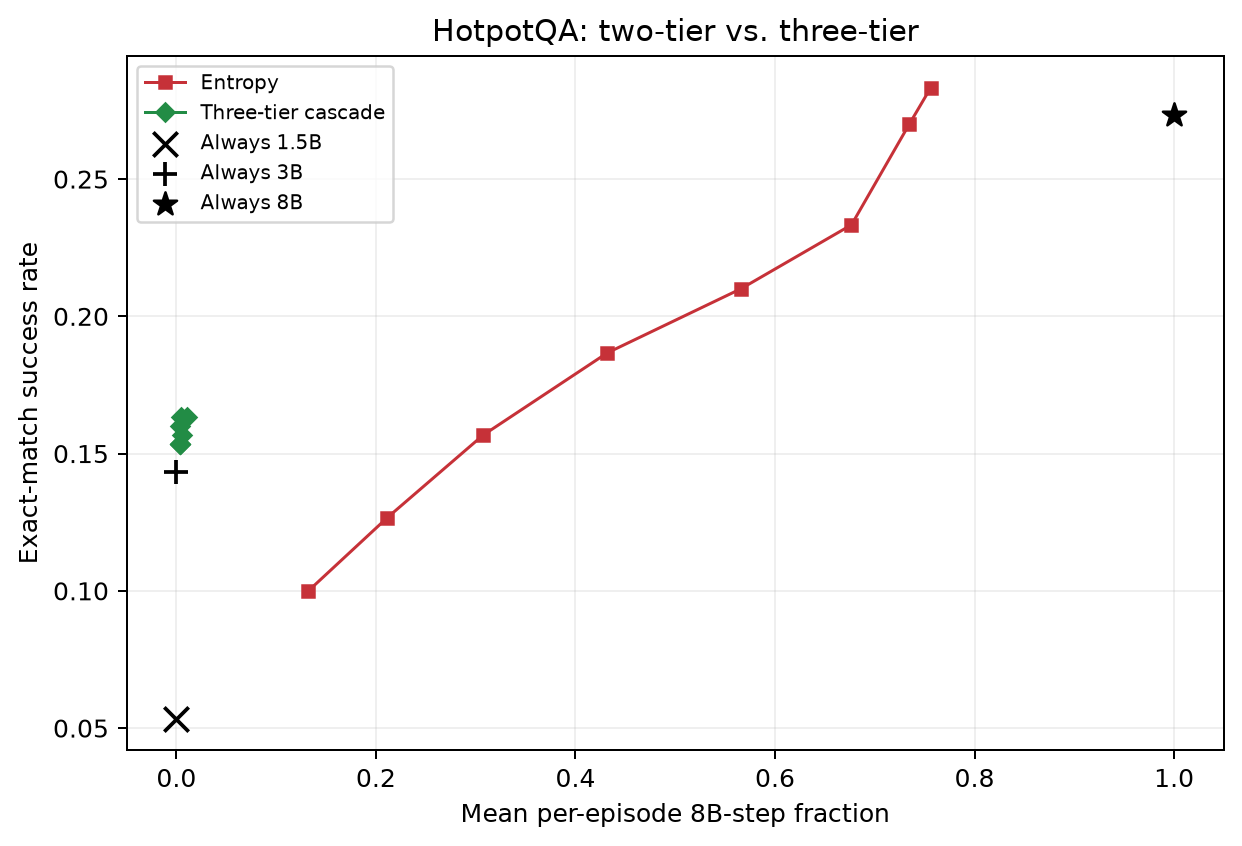
\includegraphics[width=\linewidth]{fig2_3level_vs_2level.png}
  \caption{Three-level cascade vs. two-level entropy routing on HotpotQA. The
  cascade reaches 0.163 success at near-zero 8B usage. A two-level entropy
  gate reaches 0.157 success at a 0.307 mean 8B-step fraction and 0.187 at
  a 0.432 fraction. These are observed scores, not equivalence tests.}
  \label{fig:cascade}
\end{figure}

\subsection{Offline AUC Does Not Guarantee Online Routing Value}

The learned router attains training-set AUC 0.706 on logged 1.5B baseline steps, and 0.719
when step index is added as an ablation. The deployed logit-only router is
therefore discriminative on its training data, without a held-out estimate. Online, however, all learned thresholds are
Pareto-dominated within each dataset. The router has a sharp threshold cliff:
threshold 0.3 assigns nearly all executed steps to 8B, while threshold 0.4
drops to roughly 0.6 mean 8B-step fraction and
loses substantial success. This is a useful negative result: proxy labels and
logged-step discrimination do not necessarily transfer to a good online
routing policy.

Figure~\ref{fig:signal} reports a separate pooled diagnostic: first-token
entropy has AUC 0.658 and inverted top-1 probability has AUC 0.656 across
all three baseline models. These pooled values can reflect model and dataset
differences and do not estimate held-out discrimination for the 1.5B router.

\begin{figure}[t]
  \centering
  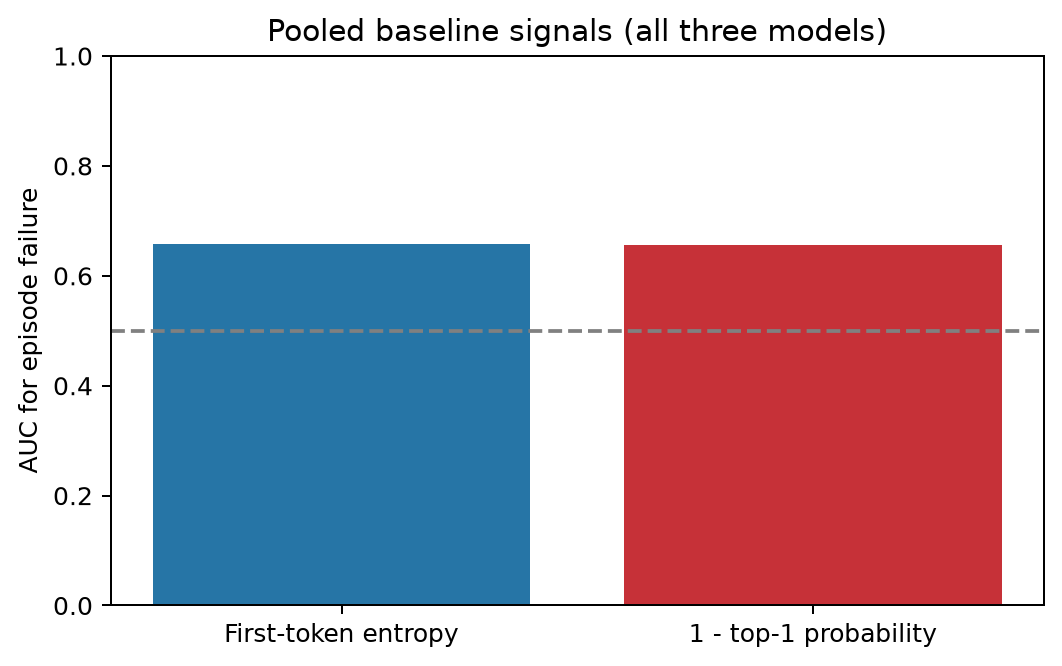
\includegraphics[width=0.8\linewidth]{fig4_signal_quality.png}
  \caption{Signal quality pooled across 6,418 steps from all three baseline
  models and both datasets. The label is episode failure, not action
  correctness. Confidence values are unavailable in these logs. This pooled
  diagnostic differs from the 1.5B-only learned-router AUC.}
  \label{fig:signal}
\end{figure}

\subsection{Cross-Task Pattern}

MuSiQue shows similar qualitative patterns (Figure~\ref{fig:mq}):
entropy gating contributes non-dominated points, confidence gating is weak,
learned routing is dominated, and cascades perform well at near-zero 8B usage.
This is a descriptive comparison across the sampled datasets, not held-out
cross-task generalization: the learned router was trained on both.

\begin{figure}[t]
  \centering
  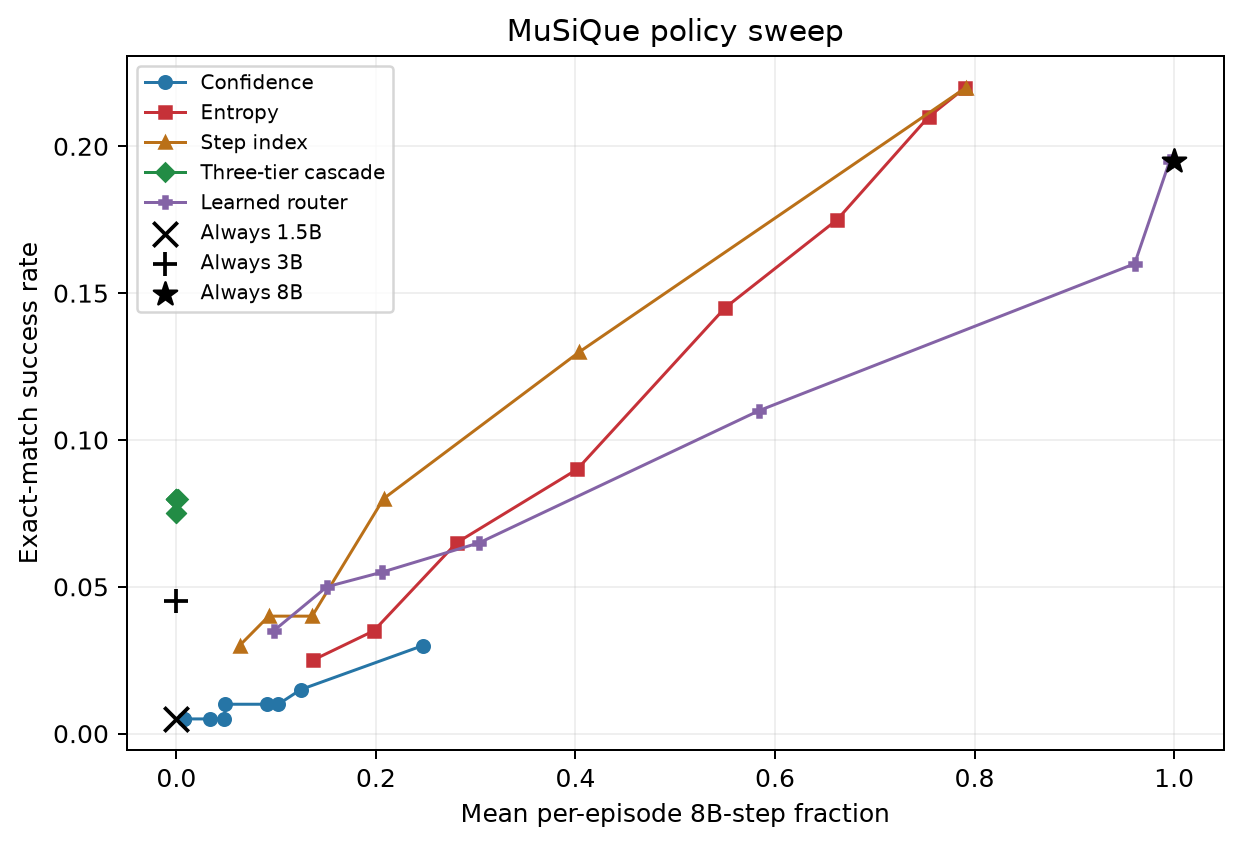
\includegraphics[width=\linewidth]{fig5_cross_task.png}
  \caption{MuSiQue policy sweep. Entropy contributes non-dominated points,
  learned routing is dominated, confidence gating is weak, and cascades
  improve observed accuracy over always-3B at very low 8B usage.}
  \label{fig:mq}
\end{figure}

\section{Discussion}

The main lesson is that agent routing should be evaluated as a trajectory-level
intervention. Entropy gating improves observed accuracy at higher 8B usage, but a ReAct episode succeeds
only if the sequence of actions, observations, and termination decisions works
together. The sweep does not isolate which individual interventions cause success or failure.

The strength of the step gate suggests that not all positions in a trajectory
are equally valuable. One hypothesis is that initial search is easier than subsequent evidence use
and answer formation. The entropy pattern is consistent with this hypothesis,
but could also reflect formatting or trajectory selection. Correctness
annotations and controlled interventions are needed to distinguish these explanations.

The cascade result motivates testing intermediate models as an alternative
to direct 1.5B-to-8B routing. Our 3B baseline is more accurate than the
1.5B baseline, but its hardware-dependent
inference cost was not measured. Low 8B usage does not establish overall efficiency.

Finally, the learned-router result is a warning for offline evaluation.
Step-level labels derived from episode success are noisy: a step from a failed
episode is not necessarily the step that caused failure, and an online router
changes the future state distribution. AUC on logged steps is therefore an
insufficient success criterion.

\section{Limitations}

This study uses 300 HotpotQA and 200 MuSiQue questions. The sweep is broad,
but some pairwise differences, especially cascade improvements over the 3B
baseline, require larger confirmatory runs. We therefore frame those results
as frontier structure rather than definitive effect-size claims.

The cost proxy reports mean per-episode 8B-step fraction, not total compute. Because the router
uses a generate-then-route design, every escalated step also incurs a 1.5B
generation, and cascade steps may incur 1.5B and 3B generations before an 8B
call. Confidence gates incur another SLM call to elicit a score. Future versions
should log every invocation, input/output tokens, and measured GPU time.

The learned router is trained and evaluated on the same 500 questions.
All thresholds are compared on these questions, so best thresholds are
exploratory selections rather than held-out estimates. The learned router
also uses episode-level proxy labels rather than step-level causal labels. This is realistic for many logging settings but imperfect:
failed episodes may contain correct steps, and successful episodes may contain
steps that only succeeded because later steps recovered.

The environment is a controlled BM25-over-candidates QA setting, not open-web
search. This makes routing behavior easier to audit but does not cover all
agent deployments. The reference is an 8B open-weight model, not a frontier closed model.
Our exact-match implementation checks one gold answer string and does not
implement all official benchmark metrics or answer-alias handling.
Model size and family are confounded between Qwen and Llama. Finally, all decoding is greedy and all main results use one SLM
family, so the conclusions should be tested with additional model families and
sampling regimes.

\section{Conclusion}

Per-action routing is a useful abstraction for ReAct agents, but the empirical
picture is more nuanced than simply escalating uncertain steps. In our
multi-hop QA setting, entropy gating is competitive while the tested
confidence gate is weak; a learned router with training-set AUC 0.71 fails to produce a
competitive online policy; and simple structural policies explain much of the
recoverable value. Two separately evaluated policies merit follow-up: escalation after the
first action gives similar observed accuracy to always-8B, and a mid-tier
cascade gives higher observed accuracy than always-3B with little 8B use.
Their combination and total compute savings remain untested. These findings support a cautious, measurement-first approach to
cost-aware routing in language-agent systems.

\bibliographystyle{ACM-Reference-Format}
\bibliography{references}

\end{document}
